\documentclass[12pt]{article}

\usepackage[utf8]{inputenc} % utf8 is the default in modern LaTeX distributions
\usepackage{amsmath}
\usepackage{fancyhdr}
\usepackage{indentfirst}
\usepackage{geometry}
\usepackage{setspace} 
\usepackage{graphicx}
\graphicspath{{Images/}}
\usepackage{float}
\usepackage[none]{hyphenat}
\usepackage[table]{xcolor}
\usepackage{titlesec}
\usepackage[colorlinks=true,
            linkcolor=blue,
            citecolor=red,
            allcolors=blue,
            pdftex,
            pdfpagelabels=true,
            hypertexnames=false]{hyperref}
\usepackage[all]{hypcap}
\usepackage[noabbrev]{cleveref}



\geometry{left=1in,right=1in,top=1in,bottom=1in}

% Custom title page design
\renewcommand{\maketitle}{
    \thispagestyle{empty}
    \begin{center}

    
    % University header
    \normalsize
    University of California Santa Cruz \\
    Baskin School of Engineering \\
    Electrical and Computer Engineering Department
    \vspace{1.5cm}

        
    % University logo
    
\includegraphics[width=0.4\linewidth]{Images/UC-Unofficial-seal.jpg}
    \vspace{1.5cm}
    
    % Report title
    \Huge\bfseries
    Wet/Dry Cycling Final Report
    \vspace{1cm}
    
    % Authors
    \large
    Rafael Delwart, Cole Schreiner, Matthew Randall, \\
    Ryan Taylor \& Ana Villa
    \vspace{1cm}

    
    % Course info
    \normalsize\normalfont
    ECE 129 \\
    Instructor: Stephen Petersen \\
    TA: Evripides Nicolaides
        
    % Date
    \normalsize\normalfont
    26 May 2025
    \vspace{2cm}
    
    \end{center}
    \newpage
}

\begin{document}
\maketitle  % This now generates the complete title page

% New page for the rest of the content
\newpage
\pagestyle{fancy} % Set page style to fancy for the rest of the pages
\fancyhead[R]{\thepage} % Add page number to the top right
\fancyfoot{} % Clear default footer
\setcounter{page}{1} % Start page numbering from 1

\doublespacing

% Removes LaTeX 'Contents' header line
\renewcommand{\contentsname}{}  % Remove default LaTeX title
% \begin{centering}
\section*{\centering{Table of Contents}}
% \end{centering}
\tableofcontents


\newpage




\section{Abstract}
    

\section{Introduction}
% \begin{spacing}{1} % Sets spacing to 1.5 inside this block

    The prevailing scientific theory of the origins of life proposes that life began in the ocean, where hydrothermal vents provided the necessary energy and chemical gradients for the first biomolecules to form. However, Professor David Deamer is challenging this ocean-centric model by proposing an alternative hypothesis: that life may have originated in freshwater hydrothermal pools on land, where wet-dry cycles played a critical role in driving prebiotic chemical reactions. Unlike the deep ocean, these terrestrial environments would have allowed for periodic dehydration and rehydration, which Deamer argues is essential for the polymerization of RNA. 
    
    Deamer's current research suggests that wet-dry cycles in early Earth hydrothermal environments may have driven the abiotic synthesis of RNA molecules. However, experimental progress into this theory has been limited by the lack of automated systems that can precisely simulate hydrothermal environments. Through the development of a automated system to simulate hydrothermal environments, this project aims to progress the research in the role of wet-dry cycling in the theory of the origins of life. Under the guidance of Professor David Deamer, a researcher in prebiotic chemistry, the team engineered a modular system capable of simultaneously processing multiple samples with precise environmental controls. The machine features automated fluid handling, temperature regulation, gas control, and mixing capabilities, with user control over each variable. This system provides researchers with control over environmental parameters including temperature, humidity, gas composition, and cycling frequency. By automating the process of wet-dry cycling, this project aim to create a high-throughput platform that advances origins-of-life research. 
    
   
% \end{spacing}

\section{Top Level Overview}

    \begin{figure}[H]
    % [h] - "Here" (approximate)
    % [H] - Exact location (requires \usepackage{float})
    % [htbp] - LaTeX's best judgment (default recommendation)
        \centering
        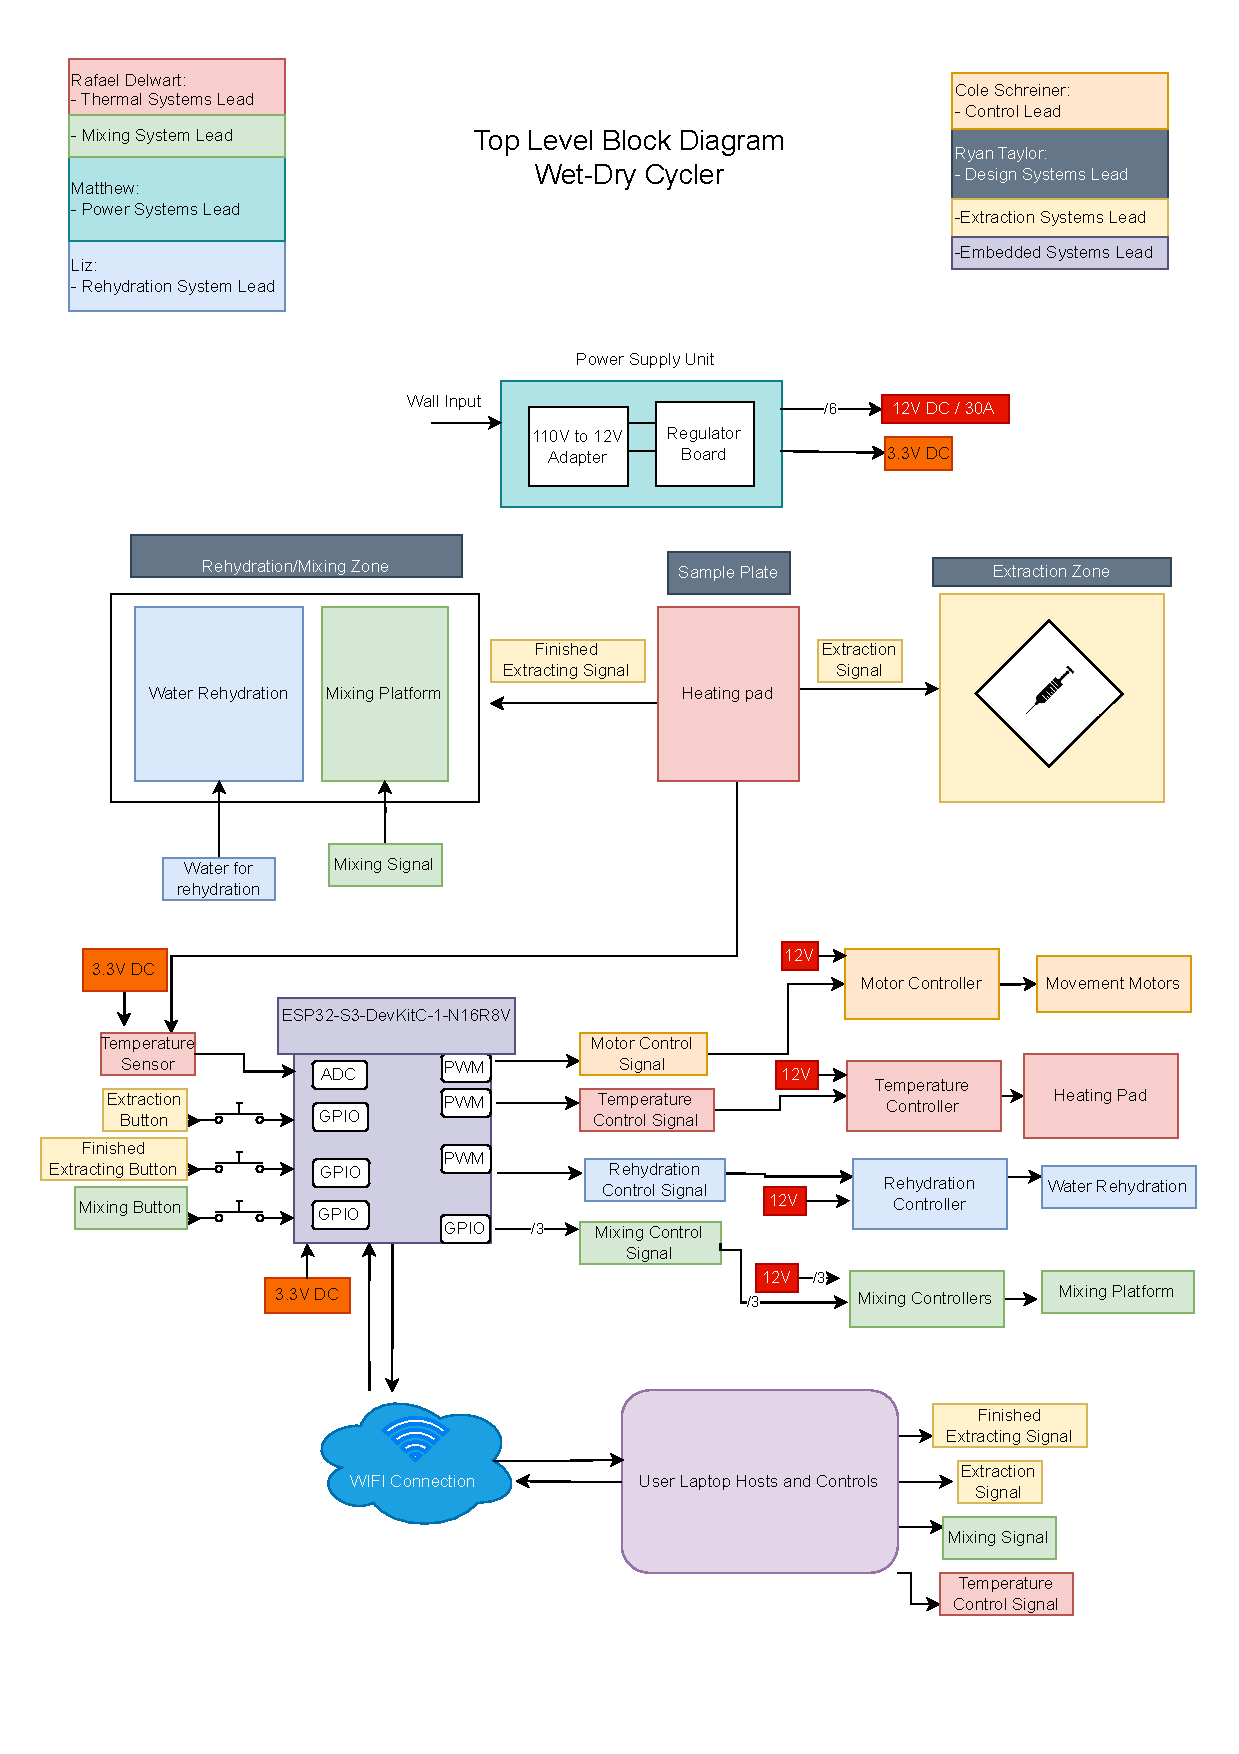
\includegraphics[width=.8\textwidth]{Top_Level_V3.1.drawio.pdf}
        \caption{Overall system block diagram}
        \label{fig:Block_Diagram}
    \end{figure}
    
    The system block diagram, shown in \autoref{fig:Block_Diagram}, provides a top-level visual representation of the wet-dry cycling machine’s architecture. The system flow from the block diagram shows that first the samples are heated using the silicon heating pad followed by sample rehydration and magnetic mixing. When the client is ready to extract the sample, the extraction button is pressed and the entire platform moves to the extraction zone. When extraction is finished the client then presses the button again and the samples go back into the wet/dry cycling. The block diagram breaks down the system into eight core functional subsystems; the temperature control module, fluid delivery system, CO$_2$/N$_2$ delivery unit, mixing mechanism, platform movement mechanism, power distribution, microcontroller design and user interface. Each block encapsulates a distinct operational domain, with standardized symbols and interconnecting arrows explicitly mapping the flow of control signals, materials, and data. This hierarchical decomposition of the overall system enabled the team to break down the project and assign sub-team leads. 

    The Wet-Dry Cycler project was organized into six subteams: thermal systems, mixing systems, movement systems, power/electrical, mechanical integration, and fluid delivery. Each subteam was responsible for a distinct subsystem that contributed to the overall functionality and reliability of the device.

   The thermal systems subteam oversaw temperature regulation throughout the dry phase of the cycle. This included implementing a system capable of reaching and maintaining target temperatures with precision within 5$\,^\circ\mathrm{C}$ to support consistent sample drying. The team was also responsible for integrating feedback mechanisms to monitor thermal behavior and ensure the repeatability of heating operations across multiple cycles.

    The mixing systems subteam managed the design and operation of the agitation platform, which was responsible for uniformly mixing fluid into samples during the wet phase. The subteam goal was to ensure thorough and repeatable mixing to promote sample integrity prior to extraction. 
    
    The movement systems subteam developed the actuation mechanisms that enabled sample transport between the preparation and extraction zone. The subteam's responsibilities included establishing the motion sequence, designing the interface between the control unit and motors, and ensuring reliable positioning within 10mm. This functionality was critical for automating transitions and enabling the continuous operation of the wet-dry cycle.
    
    The power and electrical subteam was responsible for the electrical infrastructure of the system, including power distribution, voltage regulation, and circuit design. The subteam was tasked with creating a power system to power every component reliably. The team also was tasked with creating an engineering schematic of the entire electrical system and making a PCB to deliver all microcontoller signals reliably. 
    
    The mechanical integration subteam focused on the physical layout and structural assembly of the device. They ensured that all subsystems—thermal, electrical, mixing, movement, and fluid—were securely mounted and spatially coordinated within the system enclosure. In addition to managing the overall structural framework, this subteam was responsible for designing and implementing the CO\textsubscript{2} delivery system, which introduced controlled amounts of gas into the chamber as part of the dry phase. Their work supported subsystem alignment, ease of maintenance, and reliable overall operation.
    
    The fluid delivery subteam designed the rehydration subsystem to deliver controlled volumes of fluid to the sample plate during the wet phase. Their work involved integrating fluid flow components with control hardware and coordinating timing with the mixing platform. The team prioritized consistent delivery, minimal leakage, and compatibility with the surrounding mechanical and electrical systems.

    
    \section{Subsystem Overview}

    \section{Containment}

    \section{Electrical System}

        The electrical system was designed to meet three primary objectives: ensure reliable power delivery to all components, establish a robust internal wiring architecture within the enclosure, and develop a dependable signal transmission system for control logic. To address these goals, this report is divided into two main sections: the power delivery system and the overall circuit design.
    
    \subsection{Power System Design}
    
        The power system was developed to provide stable and efficient voltage levels required by all electrical subsystems. It was essential to ensure reliable operation under varying load conditions. The power system was designed using a top-down approach: a power budget was created to understand the system’s load requirements, a power system block diagram was developed to establish the overall architecture and an engineering schematic was produced to validate the design and support testing.
    
    \subsection{Power Budget and Load Requirements}
    
        To ensure reliable operation of all subsystems, a power budget was developed to characterize the system’s electrical demands.\footnote{See Appendix for linked power budget} The analysis considered each component's voltage requirements, current consumption across different states, and total energy usage over a 24-hour duty cycle. 
        
        
        The heating pad represents the dominant power load in the system, accounting for the vast majority of total energy consumption. Operating at 12V, it requires 17.6A, necessitating careful consideration of both power regulation and thermal management. In addition, multiple motors—including NEMA 17 stepper motors and brushless DC motors—contribute significant current draw, ranging from 50mA to 2A, during active states. These components require high instantaneous current and introduce spectral noise that must be managed through proper isolation and grounding strategies. It's important to note that the two stepper motors for rehydration and movement systems will never be in high states simultaneously.
        
        Due to the high current demands of components such as the heating pad, stepper motors, and motor drivers, a 12V power supply was selected to serve as the primary voltage source. This choice was based on its ability to meet the system’s load requirements while maintaining voltage within the acceptable input ranges for all downstream regulators and devices. The power supply was experimentally measured to deliver stable a 12V operating up to 25A with 1.6\% error in voltage.
    
    \subsection{Power System Block Diagram}




    \section{Website}
        % \section{Web Interface}

            The web interface is a critical component of our wet/dry cycling system. It is designed to provide researchers with a user-friendly and reliable method of interacting with the hardware. The primary purpose of this web platform is to allow our client, an academic researcher in biomolecular engineering, to view, configure, and log experimental parameters related to RNA synthesis. Our interface simplifies the complexity of the underlying hardware and provides a clear, structured interface through which experiments can be initiated, monitored, and controlled.
            
            \subsection{Purpose and Role in System Architecture}
            
            The web interface serves as the primary bridge between the user and the hardware controller, enabling real-time interaction during RNA wet/dry cycling experiments. The site is designed to facilitate three main objectives:
\begin{itemize}
    \item Setup system state and experimental parameters
    \item Direct manipulation and configuration of experiment settings (e.g., temperature, timing, pump actuation)
    \item Resilient state tracking in the face of power loss or accidental disconnections
\end{itemize}
It enables experimenters to conduct cycles with fine control while minimizing the need for direct hardware interaction.
            
            \subsection{Technological Stack}
            
            The web system is composed of several tools and frameworks:
            
            \begin{itemize}
                \item \textbf{React.js (Frontend)} — A component-based JavaScript library used to build an interactive, responsive interface.
                \item \textbf{Node.js (Backend Server)} — A JavaScript runtime used to serve the site and maintain a persistent WebSocket connection with both the browser and the ESP32 microcontroller.
                \item \textbf{WebSocket Protocol} — Enables bidirectional, real-time communication between the frontend, backend, and ESP32. This is essential for maintaining synchronization between user commands and system state.
                \item \textbf{ESP32-S3 (Hardware Controller)} — Communicates via WebSocket with the Node.js server to receive instructions and report internal state.
                \item \textbf{JSON-Based State Recovery System} — A local file system mechanism used to record system state, allowing state persistence across frontend reloads and microcontroller resets.
            \end{itemize}
            
            \subsection{Key Features and Design Considerations}
            
            Throughout the development process, particular emphasis was placed on safety, robustness, and clarity in the interface design. The following features were central to the final implementation:
            
            \subsection{State Machine Interface}
            
            A dynamic state machine was developed and embedded into the frontend logic. This state machine mirrors the internal state of the ESP32 and ensures that both systems agree on the current operational mode (e.g., Setup, Priming, Cycling, Complete). The frontend is responsible for transitioning between interface states only when mutual confirmation from the ESP32 is received, ensuring synchronization and reducing the risk of invalid or conflicting user actions.
            
            \subsection{Tab-Based Input Access}
            
            To enforce a clear and controlled workflow, the interface is organized into tabbed sections. Each tab quarantines a different set of user inputs and options corresponding to specific stages of the wet/dry cycling process. Inputs are conditionally locked or unlocked based on the current state of the experiment. For example, parameter fields are editable only during the setup state, and unavailable once a cycle begins. This “walled garden” approach significantly reduces the possibility of user error and enhances safety.
            
            \subsection{Robust Recovery and State Persistence}
            
            One of the most important aspects of the system is its ability to persist state across disruptions. We implemented a JSON-based state recovery mechanism that records the current frontend and backend state to disk. Upon reloading the web page, the frontend queries the backend for this state and re-enters the exact interface state present before reload or power loss. Similarly, the ESP32 retains its state through local storage and resumes operation coherently after resets. This design ensures that experiments are not disrupted by power interruptions or accidental browser closures.
            
            \subsection{Real-Time Feedback and Logging}
            
            The frontend continuously displays the current state of the hardware and relevant telemetry, such as temperatures, timing cycles, and pump status. Any change made by the user is immediately reflected in the system and logged. This real-time interactivity is enabled by the persistent WebSocket connection, which minimizes latency and keeps the interface in sync with the hardware.
            
            \subsection{Challenges and Development Journey}
            
            The development of the web interface posed several technical and conceptual challenges, especially given the team’s limited prior experience with full-stack web development.
            
            \subsection{Learning Curve}
            
            The process began with an extensive exploration of available tools and frameworks. Choosing React and Node.js involved a tradeoff between complexity and capability. As no team members had formal training in JavaScript or web design, significant time was invested in learning fundamental concepts, including asynchronous communication, component lifecycles, and frontend-backend interactions.
            
            \subsection{State Management and Synchronization}
            
            A particularly difficult problem was ensuring agreement between the frontend UI state, backend server state, and microcontroller state. We explored multiple paradigms for shared state and eventually settled on a file-based persistence system that could be accessed by both frontend and backend on reload. Considerable effort was spent debugging edge cases where components could fall out of sync, especially during power loss scenarios or user-initiated reloads.
            
            \subsection{UI Logic and Safety Constraints}
            
            Creating a clear, intuitive, and constrained user experience proved to be as challenging as the technical backend. JavaScript’s asynchronous behavior, nested callback logic, and rendering rules often made it difficult to enforce strict control flow. Interface elements had to be rearranged multiple times to satisfy both usability and safety constraints. We introduced conditional rendering and state-locked components to prevent invalid operations from being sent to the ESP32 at inappropriate times.
            
            \subsection{Design Evolution and Final Implementation}
            
            Over the course of three academic quarters, the web interface evolved from a simple serial logger into a robust, safety-oriented experiment control panel. Early versions used raw HTML and ad hoc communication protocols, but were quickly replaced with a more maintainable and modular React architecture. As our understanding of real-time systems deepened, we introduced the state machine framework and implemented rigorous testing to verify state integrity under all circumstances. 
            
            The final interface is tightly integrated into the overall system and designed to be maintainable and extensible. Although the system is currently run locally via \texttt{localhost}, the architecture would support deployment to a remote server with minimal changes, allowing remote experiment control and data collection.
            
            \subsection{Conclusion}
            
            The web interface successfully meets the goals of providing a safe, user-friendly, and recoverable platform for managing RNA wet/dry cycling experiments. It represents a substantial technical achievement for the team, requiring integration of full-stack development, hardware communication, and human-computer interaction principles. The final system enables precise experimental control, even under failure conditions, and serves as a solid foundation for future extensions such as remote access or automated data analytics.



    
    
    \section{Heating}
    
    \section{Mixing}
    
    \section{Rehydration - Contributors: Ana Villa}
        The objective of this experiment was to evaluate the accuracy and consistency of a custom-built rehydration system, which distributes water from a syringe pump through a 13-port manifold into twelve separate output channels. The system was designed to deliver approximately 100 microliters (µL) of water per outlet for each cycle. This study aimed to assess the precision of volume delivery using resource-limited tools and to suggest hardware improvements based on observed performance.
        
        \subsection{Materials and Methods}
        A syringe pump was used to drive deionized water into a 13-port manifold. The setup involved a 25 mL syringe connected to the single intake port of the manifold, while the remaining twelve ports served as outputs. Each output line was connected to a short segment of tubing ending in a manual valve, which allowed control over flow to the collection containers and helped prevent unwanted dripping or air intake. Prior to testing, all tubing and ports were pre-filled with water to remove air bubbles and ensure consistent flow at the start of each run.
        
        Due to constraints in funding and access to precision equipment, a manual 20–200 µL pipette was used to measure the amount of water delivered by each port. After one full distribution cycle (approximately 1.2 mL total from the syringe pump), water was manually drawn from each output using the pipette and recorded. This process was repeated over multiple cycles to evaluate average performance, with each reading compared against the expected 100 µL target.

    \subsection{Test and Results}
    \begin{figure}[H]
        \centering
        \includegraphics[width=1\linewidth]{Screenshot 2025-05-23 at 3.34.58 PM.png}
        \caption{Water Port Test 1}
        \label{fig:enter-label}
    \end{figure}
        The system delivered water to all twelve output ports with an average volume close to 100 µL per port. Across several trials, the average percent error was determined to be approximately 8 percent. The highest observed deviation from the target volume was 13 percent, while the lowest was 4 percent. The measurements, though manually performed and subject to slight user variability, provided a reasonable indication of system performance given the constraints.
    
    
    \subsection{Discussion}
        The results demonstrate that the rehydration system performs reliably within the target range for most general-purpose applications. Pre-filling the tubing and including valves at the outputs were crucial to achieving this level of consistency, as they eliminated major sources of variability such as trapped air and inconsistent pressure. Using a pipette for volume measurement was a pragmatic solution in the absence of a precision balance and enabled effective identification of variation between outputs.
        
        While the average error was within acceptable margins for many biological protocols, tighter control may be needed in more sensitive procedures. Improvements in future iterations could include automation of the measurement process or switching to flow sensors for real-time monitoring. Additionally, to enhance mechanical performance and precision, it is recommended to adopt a more specialized syringe pump. Specifically, the SSP Series Syringe Pump with a 30 mm stroke is well-suited for this type of controlled fluid delivery. Its consistent actuation and fine control over stroke length make it ideal for small-volume distribution tasks like the one tested in this system.
    
    \subsection{Conclusion}
        The rehydration system utilizing a syringe pump and 13-port manifold demonstrated reasonably consistent water delivery of approximately 100 µL per port, with an average error of 8 percent and a range of 4 to 13 percent. The use of pre-filled tubing and manual valves contributed significantly to reducing variability. Despite limited access to precision instrumentation, the use of a pipette provided a cost-effective method for measuring performance. Future implementations could benefit from integrating a high-precision pump such as the SSP Series Syringe Pump with a 30 mm stroke for greater consistency and tighter error margins. Overall, the system is effective and adaptable, especially for resource-constrained laboratory environments.
    
    \section{Extraction}
    







\section{Conclusion}

    


\section{Appendix}

\href{https://docs.google.com/spreadsheets/d/1zga7t0Z7vdd-e0fAlvdngkhm1gBsFoFq/edit?usp=sharing&ouid=111594997472455245073&rtpof=true&sd=true}{1. Power Budget Spreadsheet}.




\end{document}




